\question \textbf{Basic measures from confusion matrix}
  
The oval representation below shows that a model has classified a test data set with 10 positives and 10 negatives and produced four outcomes.
 
\begin{figure}[H]
      \centering
      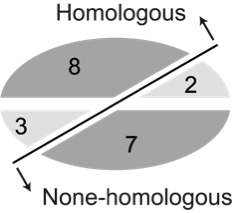
\includegraphics[width=0.2 \textwidth]{fig07/oval_representation.png}
\end{figure}

\vspace{0.1 in}

\begin{parts}

%% (a)
  \part Fill each blank cell with one of the four classification outcomes - TP, FP, TN, and FN.

\begin{table}[H]
\centering
\begin{tabular}{ll|c|c|}
\cline{3-4}
                                                            &                & \multicolumn{2}{c|}{Test data}                                        \\ \cline{3-4} 
                                                            &                & \multicolumn{1}{l|}{Homologous} & \multicolumn{1}{l|}{Non-homologous} \\ \hline
\multicolumn{1}{|l|}{\multirow{2}{*}{Model classification}} & Homologous     &                                 &                                     \\ \cline{2-4} 
\multicolumn{1}{|l|}{}                                      & Non-homologous &                                 &                                     \\ \hline
\end{tabular}
\end{table}

%% (b)
\part Make a confusion matrix from the oval representation above.

\begin{table}[H]
\centering
\begin{tabular}{ll|c|c|}
\cline{3-4}
                                                            &                & \multicolumn{2}{c|}{Test data}                                        \\ \cline{3-4} 
                                                            &                & \multicolumn{1}{l|}{Homologous} & \multicolumn{1}{l|}{Non-homologous} \\ \hline
\multicolumn{1}{|l|}{\multirow{2}{*}{Model classification}} & Homologous     &                                 &                                     \\ \cline{2-4} 
\multicolumn{1}{|l|}{}                                      & Non-homologous &                                 &                                     \\ \hline
\end{tabular}
\end{table}

%% (c)
  \part Calculate the following basic evaluation measures for the oval representation. Round off the answer to two decimal places if necessary.
  
\bigskip 
Accuracy
$= \dfrac{TP+TN}{P+N} $

\bigskip 
Error rate
$= \dfrac{FP+FN}{P+N} $

\bigskip 
Sensitivity
$= \dfrac{TP}{P} $

\bigskip 
Specificity
$= \dfrac{TN}{N} $

\bigskip 
Precision
$=\dfrac{TP}{TP+FP}$


\end{parts}

